\section{Programmiersprachen}
\setauthor{Felix Dumfarth}

\subsection{Java}

\begin{figure}[hbt!]
    \centering
    
\includegraphics[scale=0.5]{pics/java}
    \caption{Java Logo\cite{java}}
    \label{fig:impl:java}
\end{figure}

Für das Backend wurde sich für Java entschieden.
Java ist laut dem TIOBE-Index\cite{tiobe} eine der populärsten Programmiersprachen.
Java ist eine für Menschen sehr einfach lesbare Sprache, aber das Maschinen sie lesen können braucht man den Java-Compiler der den Code zu einem Java-Bytecode umwandelt.
Ohne diesen Vorgang kann der Code nicht aufgeführt werden.
Java wird mit Attributen wie Einfachheit, Vertrautheit, Robustheit, Sicherheit, Leistungsfähigkeit und Architekturneutralität assoziiert.
Java ist eine objektorientierte Programmiersprache und besitzt dadurch Klassen und Vererbung\cite{java}.
\subsection{Python}
Python ist eine Programmiersprache die mehrere Arten der Programmierung unterstützt wie zum Beispiel die objektorientierte, die aspektorientierte und die funktionale Programmierung.
Es handelt sich hier um eine Programmiersprache, die versucht einen knappen und dadurch gut lesbaren Programmierstil zu besitzen.
Dadurch das Python mit nur wenigen Schlüsselwörtern auskommt und die Syntax reduziert ist, ist eine gute Übersichtlichkeit und eine optimierte Simplizität gegeben.
Python wird oft für Machine Learning verwendet, auch bei uns kommt Python bei Rasa zum Einsatz.
Zum einen ist Rasa ein Python framework zum anderen werden die Custom-Actions mit Python umgesetzt.

\subsection{Typescript}
Typescript ist eine im Jahr 2012 von Microsoft entwickelte Programmiersprache, die eine kompakte und einfache Syntax zur Programmierung von Webseiten und Anwendungen bietet.
Typescript baut auf Javascript auf und hilft zum Beispiel beim frühzeitigen Erkennen von Fehlern.
Bei TypeScript wird mit Unterstützung von Modulen das Kapseln von Klassen, Interfaces, Funktionen und Variablen in eigene Namensräume ermöglicht.
Es gibt hierbei eine Unterscheidung von internen und externen Modulen.

\section{Technologien}
\setauthor{Felix Dumfarth}

\subsection{REST Service}
REST steht für Representational State Transfer.
REST Anfragen sind CRUD – Operationen (Create, Read, Update, Delete).
Diese sind GET, POST, PUT und DELETE Requests.
Außerdem gibt es noch OPTIONS, PATCH, HEAD, TRACE
und CONNECT diese werden aber in der vorliegenden Arbeit nicht benutzt.

* Die GET Methode ist zum Abfragen da, es soll ein Request geschickt werden und nur Daten zurückgeben werden, es soll jedoch auf dem Server wohin die Anfrage geschickt worden ist nichts geschehen außer Daten lesen.

* Bei POST sollen Daten hinzugefügt werden, im Standardfall ist in der Respone der URI der neu gespeicherten Daten

* Bei PUT sollen Daten hinzugefügt werden, falls diese schon existieren werden Sie upgedatet und falls nicht, wird ein neuer Eintrag erstellt.

* Bei DELETE sollen Daten gelöscht werden.

\subsection{Quarkus}\label{quarkus}
Quarkus ist ein Framework für Java welches sich auf die REST-Service-API ausrichtet.
Das Backend\ref{sec:backend} wurde mit Quarkus umgesetzt.

\subsection{Angular}
Angular ist ein auf TypeScript basierendes Framework für Webseiten.
Gedacht ist es für Single Page Applications.
Unser Chat Widget\ref{sec:chat-widget} und unser Dashboard\ref{sec:dashboard} wurden mit Angular umgesetzt

\subsection{Angular Elements}\label{subsec:angular-elements}
''Webkomponenten sind eine Gruppe von Web-Technologien, die es ermöglichen, benutzerdefinierte, wiederverwendbare HTML Elemente zu erstellen, deren Funktionalität gekapselt ist und damit vollständig getrennt von anderem Code.''\cite{webcomponents}

Um unsre Chatkomponente auf die Wordpress Seite zu bringen, wurde entschieden, dass die Komponente mithilfe von Angular Elements als Webkomponente exportiert wird um somit eine einfache einbindung auf die Schulhomepage zu ermöglichen.

Eine Webkomponente wird in Angular Elements in 3 Javascript Files erstellt und zwar

\begin{itemize}
    \item main.js
    \item polyfills.js
    \item runtime.js
\end{itemize}

Diese können jedoch ohne bedenken zu einem einzelnen Javascript File zusammengefasst werden.

Um die Webkomponente in HTML zu benutzen, muss man alle JS files einbinden und schon kann man seine eigene Komponente wie jedes andere Element benutzen.
\begin{lstlisting}[language=html,label={lst:webcomponent},caption={HTML File}]{HTML File}]
...
<name-der-komponente></name-der-komponente>

<script src="./runtime.js"></script>
<script src="./polyfills.js"></script>
<script src="./main.js"></script>
...
\end{lstlisting}

\section{Werkzeuge}
\setauthor{Felix Dumfarth}

\subsection{Rasa X}\label{subsec:rasa-x}
Rasa X ist ein Werkzeug um Conversation-Driven Development\ref{cdd} in die Tat umzusetzen\cite{rasax}.
Rasa X liegt über Rasa und liefert dadurch erweiterte Funktionalitäten, die man nur mit Rasa alleine nicht hätte.
Rasa X wurde mit Docker Compose\cite{rasaxDocker} auf der VM installiert\ref{sec:systemarchitektur}.

Rasa X kommt mit einer grafischen Weboberfläche, auf dieser kann man sich seine Intents, Responses und so weiter verändern und ansehen.
Man kann auch sein Model trainieren oder ein Model hochladen.

Da jedoch unser eigenes Dashboard verwendet wird, wird die grafische Oberfläche nicht benötigt, sondern nur die erweiterte Funktionalität die auch über die API aufgerufen werden kann.

Damit unser Frontend auf Rasa, welches eine Ebene unter Rasa X liegt, zugreifen kann, muss das automatisch erstellte credentials.yml file bearbeitet werden:

\begin{lstlisting}[language=yaml,label={lst:rasaXCred},caption={credentials.yml}]{credentials.yml}]
rasa:
url: ${RASA_X_HOST}/api
rest:
\end{lstlisting}

Etwas für das sehr viel Zeit in anspruch ging, war es wie es möglich ist das Rasa X mit https lauft.

Es wird ein Zertifikat benötigt, es ist möglich sich ein Zertifikat zu erstellen mithilfe des Certbots\cite{certbot}, diese Zertifikate müssen dann in den certs Ordner gegeben werden.

\begin{lstlisting}[language=bash,label={lst:certbot},caption={Install certbot and create certificates}]{certbot}]
sudo ln -s /snap/bin/certbot /usr/bin/certbot
sudo certbot certonly -d vm45.htl-leonding.ac.at
sudo cp /etc/letsencrypt/live/vm45.htl-leonding.ac.at/privkey.pem /etc/rasa/certs/
sudo cp /etc/letsencrypt/live/vm45.htl-leonding.ac.at/fullchain.pem /etc/rasa/certs/
sudo chmod 640 certs/privkey.pem
\end{lstlisting}

Außerdem müssen beim nginx server noch diverse Einstellungen vorgenommen werden.
In dem File "nginx-config-files/rasax.nginx.template" muss die Zeile mit ``include'' auskommentiert werden.
\begin{lstlisting}[language=yaml,label={lst:rasaxnginxtemplate},caption={rasax.nginx.template}]{rasax.nginx.template}]
...
server {
    listen            8080;
    include           /etc/nginx/conf.d/ssl.conf;
    ...
\end{lstlisting}

Und in ``nginx-config-files/ssl.conf.template'' müssen folgende Zeilen auskommentiert werden:
\begin{lstlisting}[language=yaml,label={lst:sslconftemplate},caption={ssl.conf.template}]{ssl.conf.templatte}]
listen                  8443 ssl;

# server_name           example.com;
ssl_certificate         /etc/certs/fullchain.pem;
ssl_certificate_key     /etc/certs/privkey.pem;
\end{lstlisting}

Nun muss Rasa X gestoppt und wieder hochgefahren, werden um die neuen Einstellungen zu übernehmen.

\subsection{IntelliJ IDEA}
IntelliJ ist ein IDE welche eine Vielzahl von Programmiersprachen unterstützt und hauptsächlich für diese Arbeit verwendet wird.

\subsection{GitHub}
GitHub ist ein online Git Repository welches die gemeinsame Programmierung von Programmierern und Entwicklern erleichtert.

\subsection{GitHub Actions}\label{subsec:github-actions}
Mit Github Actions kannst du Workflows für dein Github Repository erstellen.
Ein Workflow besteht aus einem oder mehreren Jobs, wobei ein Job aus einem oder mehreren Schritten besteht.

\begin{figure}[hbt!]
    \centering
    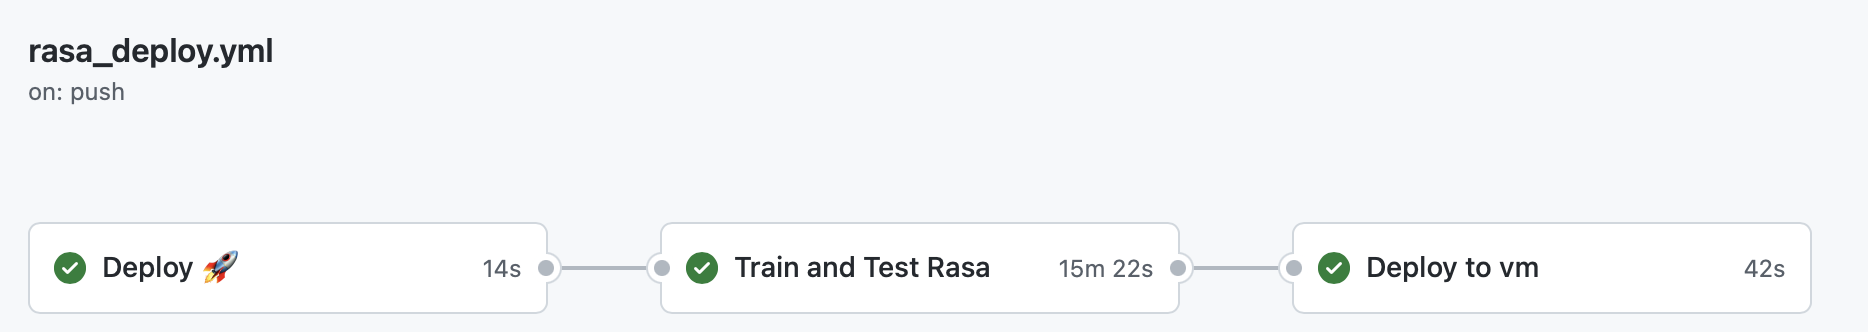
\includegraphics[scale=0.5]{pics/ghActions}
    \caption{Beispiel eines Workflows}
    \label{fig:impl:ghActions}
\end{figure}

Die Jobs werden abgearbeitet, meistens wird richtung Ende des Workflows das Produkt wohin ge-pushed.

Bei jeder Action wird Standardmäßig Checkout benutzt:

\begin{lstlisting}[language=yaml,label={lst:checkout},caption={In der Action}]{In der Action}]
...
jobs:
  build:
    runs-on: ubuntu-latest
    steps:
      - name: Checkout
        uses: actions/checkout@v2
...
\end{lstlisting}

Checkout sorgt dafür das der Workflow auf das Projekt zugreifen kann.

\subsection{Docker}
Docker ist ein Container-Manager, dies erlaubt dir Anwendungen zu Isolieren in sogenannten DockernContainern.

\subsection{Wordpress}
WordPress ist ein freies und open-source Content-Management-System, das in PHP geschrieben ist.
Für die Speicherung der Daten wird entweder eine MySQL oder eine MariaDB Datenbank verwendet.
WordPress verwendet Plugins für die Erweiterung der Funktionalitäten und Themes für die Anpassung des Designs.
Das CMS wurde ursprünglich für das Erstellen von Blogs benutzt, hat sich jedoch inzwischen zu einem System für das Verwalten verschiedenster Web-Inhalte entwickelt.
Mit einem Marktanteil von 42,8\% der 10 Millionen meistbesuchten Websites ist WordPress das beliebteste Content-Management-System.

Die HTL Leonding Schulhomepage wurde mithilfe von Wordpress gemacht, deshalb war es wichtig das unser Chatbot auch mit Wordpress kompatibel ist.


\begin{figure}[hbt!]
    \centering
    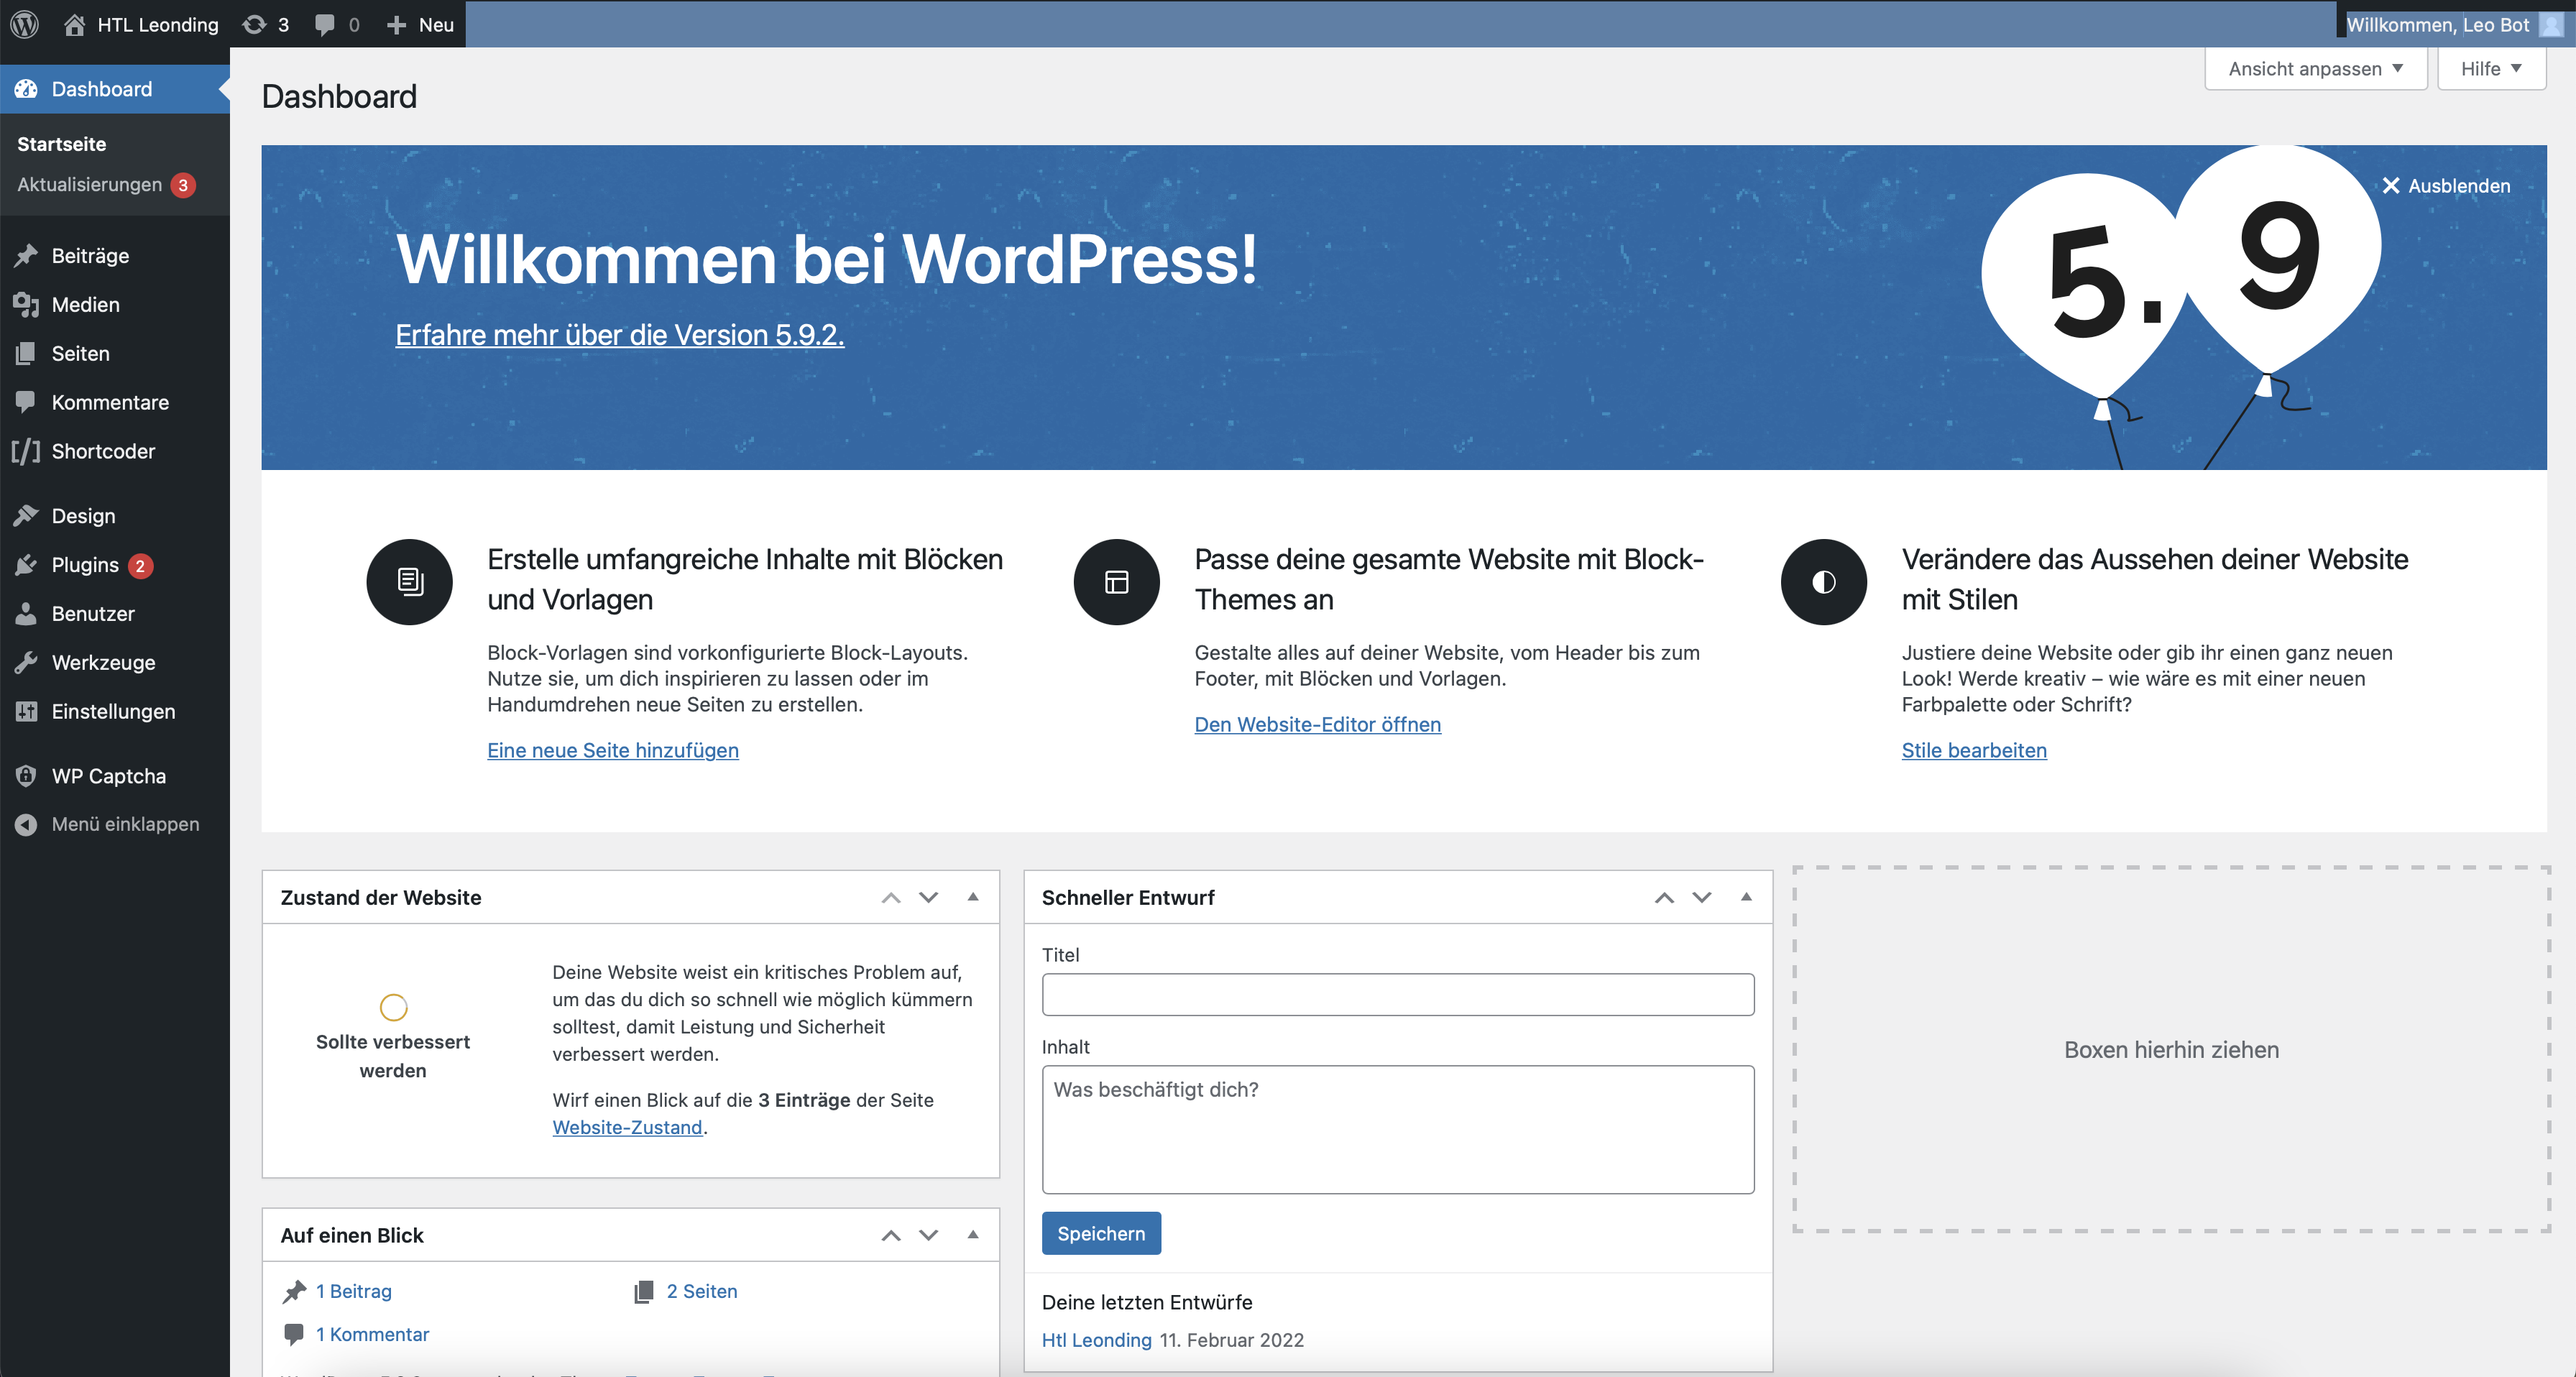
\includegraphics[scale=0.2]{pics/wordpresshome}
    \caption{Startseite Wordpress}
    \label{fig:impl:wordpresshome}
\end{figure}


Auf Wordpress kann man ganz einfach Beiträge verfassen:

\begin{figure}[hbt!]
    \centering
    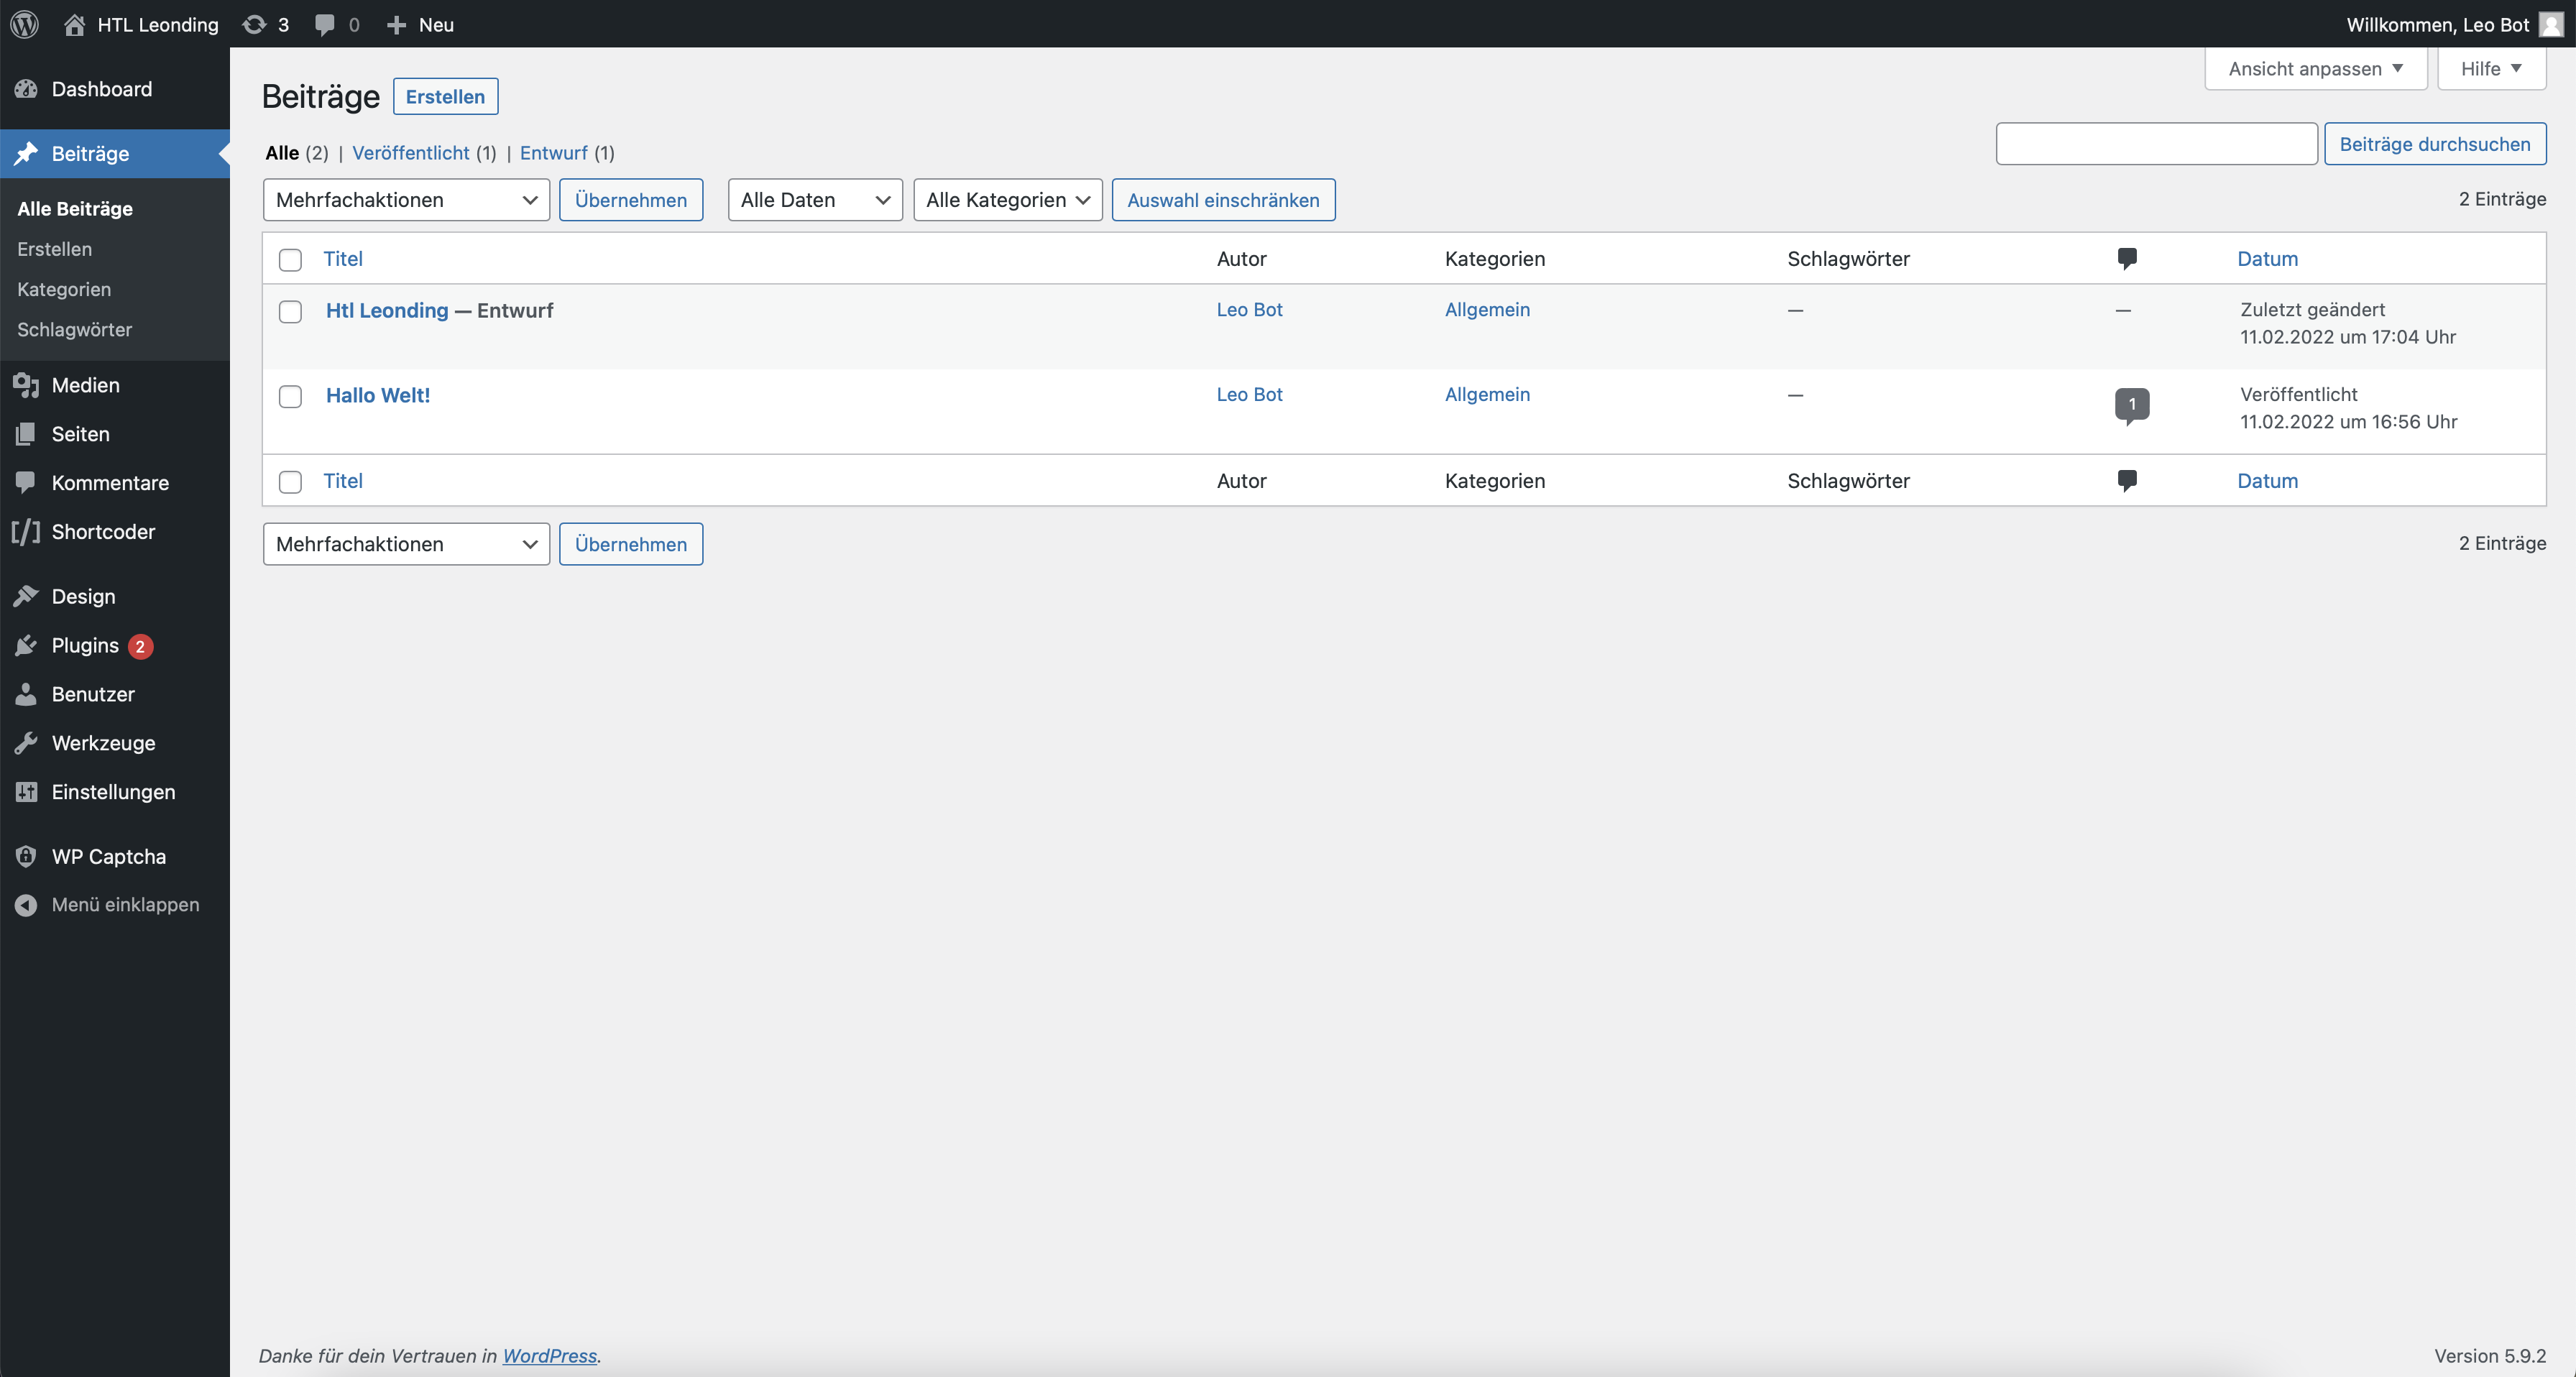
\includegraphics[scale=0.2]{pics/bloglist}
    \caption{Wordpress Liste der Blogeinträge}
    \label{fig:impl:bloglist}
\end{figure}


Diese Beiträge kann man in einem eigenen Editor, der viele vorgefertigte Elemente bereits zur Verfügung hat verfassen:

\begin{figure}[hbt!]
    \centering
    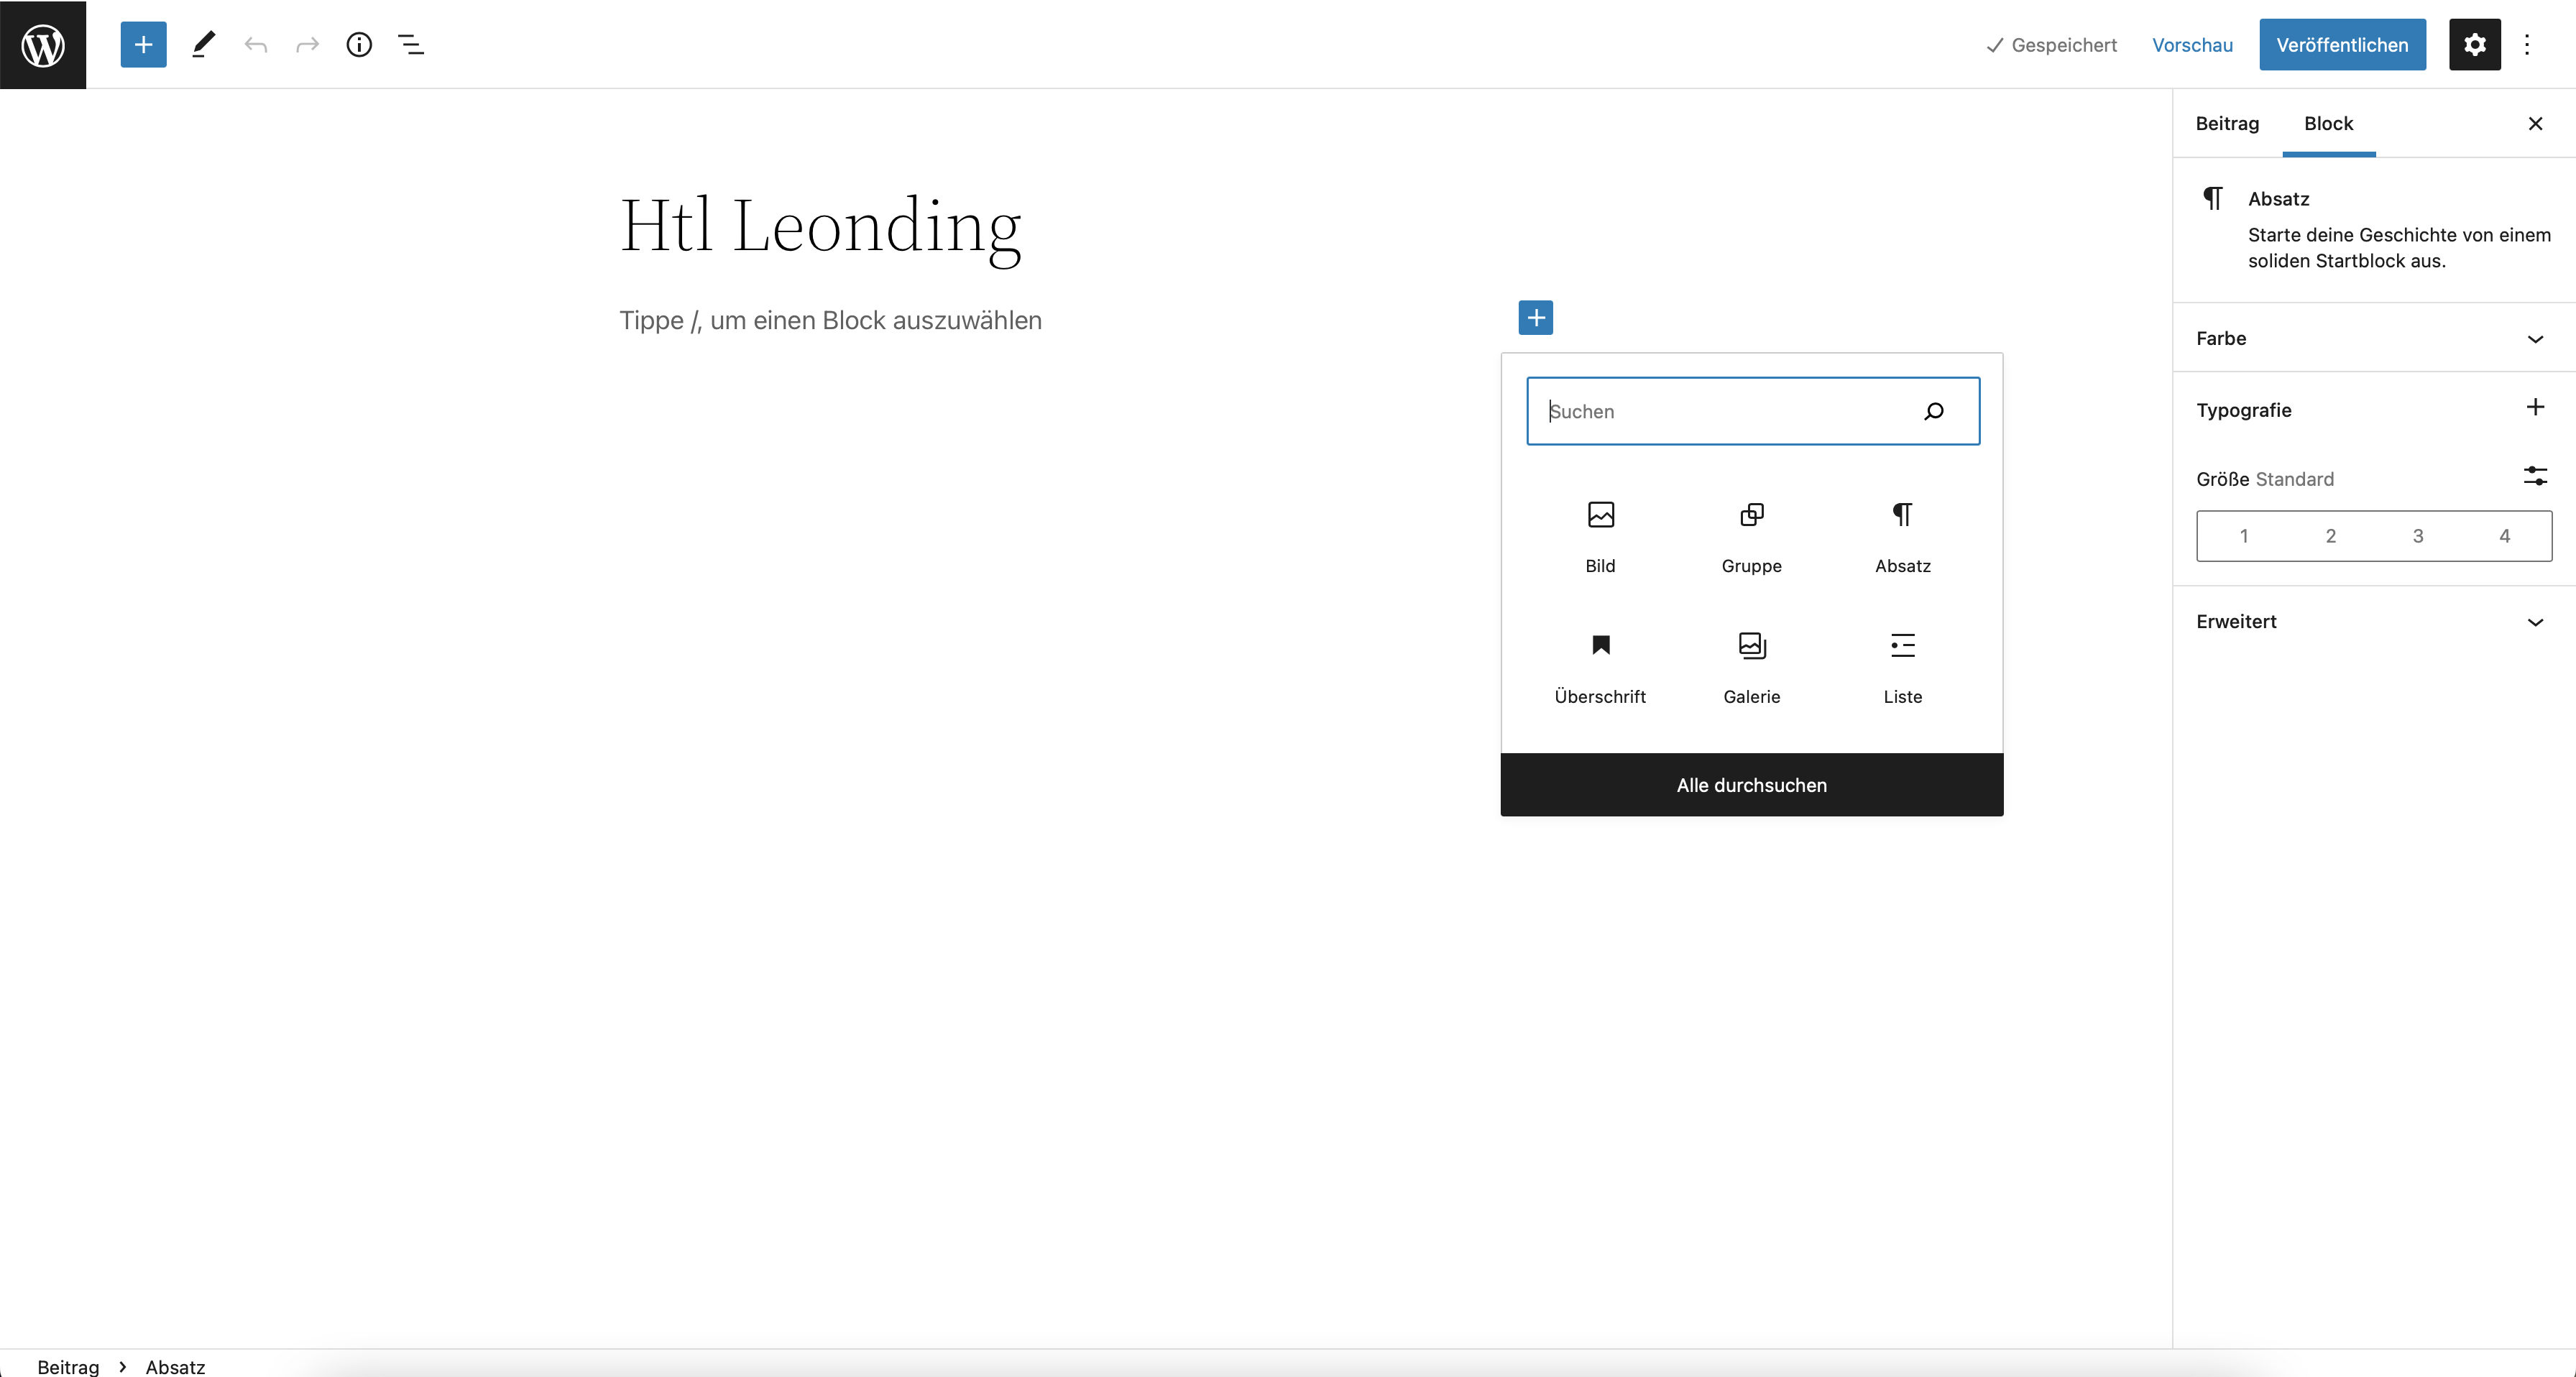
\includegraphics[scale=0.2]{pics/blogpost}
    \caption{Wordpress Blopost Editor}
    \label{fig:impl:blogpost}
\end{figure}
